\documentclass[12pt]{article}
\usepackage{hippoidP}
\usepackage{standalone}
\usepackage{dirtytalk}
\usepackage[T1]{fontenc}
\usepackage{tikz}
\usepackage{minted}

\usepackage{makeidx}
\makeindex
\usepackage[hyperindex]{hyperref}

\usetikzlibrary{arrows}
\usetikzlibrary{arrows.meta}
\usetikzlibrary{automata}
\usetikzlibrary{calc}
\usetikzlibrary{fit}
\usetikzlibrary{petri}
\usetikzlibrary{positioning}
\usetikzlibrary{shapes.geometric}

\usepackage[printsolution=true]{exercises}
\usepackage[margin=1.2in]{geometry}% Sets 1in margins.
\usepackage{float}
\setlength{\parindent}{0pt}

\docsetup{Category Theory / Haskell}{Programming with Categories}{April 8, 2024}

\theoremstyle{definition}
\newtheorem{definition}{Definition}[section]

\begin{document}
\begin{titlepage}
	\raggedleft{}
	{\Large Author Name\\[1in]}
	{\large The HandBook for\\}
	{\Huge\scshape Something or Other\\[.2in]}
	{\large My notes while reading Some Tome\\}
	{\large Spring 2324\\}
	\vfill
	{\itshape 2024, Not a Publishing Company, LLC}
\end{titlepage}

\tableofcontents
\pagebreak
\listoffigures
\listoftables

\section{Categories, Types, and Functions}
\subsection{Two fundamental ideas: sets and functions}

\begin{minted}{c}
int main() {
    printf("hello, world");
    return 0;
}
\end{minted}

here is some inline code \mint{python}|import this|.

% \inputminted{haskell}{../02-composition/src/Comp.hs}

\begin{figure}[H]
	\begin{center}
		\documentclass{standalone}
\usepackage{tikz}
\begin{document}
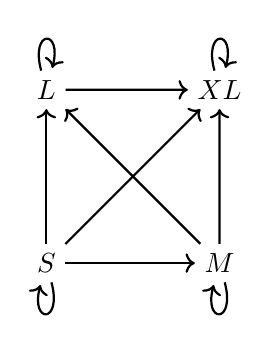
\begin{tikzpicture}[scale=1.1]
    \tikzset{arc lines/.style={thick,black, ->}}
    \node (S) at (0, 0) {$S$};
    \node (M) at (2, 0) {$M$};
    \node (L) at (0, 2) {$L$};
    \node (XL) at (2, 2) {$XL$};
    \draw [arc lines] (S) to (M);
    \draw [arc lines] (S) to (L);
    \draw [arc lines] (S) to (XL);
    \draw [arc lines] (M) to (L);
    \draw [arc lines] (M) to (XL);
    \draw [arc lines] (L) to (XL);
    \path [-stealth, thick]
        (S) edge [loop below] (S)
        (M) edge [loop below] (M)
        (L) edge [loop above] (L)
        (XL) edge [loop above] (XL)
        ;
\end{tikzpicture}
\end{document}

	\end{center}
	\caption{Toset}
\end{figure}

\printindex
\end{document}
